\section{Related Works and Countermeasures}
% \begin{figure}[h!]
%     \centering
%     \begin{minipage}{0.5\linewidth}
%         \centering
%         \begin{tikzpicture}
%             \begin{axis}[
%                 xlabel={Weight Index},
%                 ylabel={Score1/Score0},
%                 legend pos=outer north east,
%                 xmin=-1, xmax=65,
%                 font=\scriptsize,
%                 xlabel style={yshift=5pt},
%                 ylabel style={yshift=-15pt},
%                 width=1.1\linewidth,
%                 height=\linewidth,
%             ]
%                 \addplot[
%                     thick,
%                     only marks,
%                     line width=1.5pt,
%                     mark=o,
%                     mark size=1,
%                     color=darkgray,
%                     forget plot
%                 ] table {Diagrams/Data/30_min_0.txt};

%                 \addplot[
%                     thick,
%                     only marks,
%                     mark=triangle,
%                     line width=1.5pt,
%                     mark size=1,
%                     color=darkgray,
%                     forget plot
%                 ] table {Diagrams/Data/30_min_1.txt};

%                 \addplot[
%                     thick,
%                     domain=0:70,
%                     samples=2, 
%                     color=black,
%                     dashed,
%                     forget plot
%                 ] {1.13};
%             \end{axis}
%             \node[black, thick] at (1.2,3.2) {\small (a) Attack Duration: 75 minutes};
%         \end{tikzpicture}
%     \end{minipage}\hfill
%     \begin{minipage}{0.5\linewidth}
%         \centering
%         \begin{tikzpicture}
%             \begin{axis}[
%                 xlabel={Weight Index},
%                 ylabel={Score1/Score0},
%                 legend pos=outer north east,
%                 xmin=-1, xmax=65,
%                 font=\scriptsize,
%                 xlabel style={yshift=5pt},
%                 ylabel style={yshift=-15pt},
%                 width=1.1\linewidth,
%                 height=\linewidth,
%             ]
%                 \addplot[
%                     thick,
%                     only marks,
%                     line width=1.5pt,
%                     mark=o,
%                     mark size=1,
%                     color=darkgray,
%                     forget plot
%                 ] table {Diagrams/Data/75_min_0.txt};

%                 \addplot[
%                     thick,
%                     only marks,
%                     mark=triangle,
%                     line width=1.5pt,
%                     mark size=1,
%                     color=darkgray,
%                     forget plot
%                 ] table {Diagrams/Data/75_min_1.txt};

%                 \addplot[
%                     thick,
%                     domain=0:70,
%                     samples=2, 
%                     color=black,
%                     dashed,
%                     forget plot
%                 ] {1.13};
%             \end{axis}
%             \node[black, thick] at (1.4,3.2) {\small (b) Attack Duration: 30 minutes};
%         \end{tikzpicture}
%     \end{minipage}
%     \caption{Output of Thor for two different attack durations. In both figures, circles represent weights of zero, and triangles represent weights of non-zero. \textcolor{red}{TODO: instead of 30 minutes it is better to add the results for 9 minutes vs. min 50ish to show more significance difference. Also color the data points like the old figure you had was easier to see. }}
%     \label{fig:LeakedWeights}
% \end{figure}



Figure \ref{fig:thorleakage} shows \textsc{Thor} leakage rate of 76.8 bits/hour compared to other related side channels. While Platypus has a higher leakage rate, it is patched and unavailable to non-privileged users. While \textsc{Thor} does not require access to RAPL and is not limited to SGX, it exhibits a higher leakage rate compared to Hertzbleed and Collide+Power attacks.  
\textsc{Thor}'s leakage rate is {1,493\% faster than Collide+Power (MDS)} (76.8 vs. 4.82 bits/hour), and {631\% faster than Hertzbleed} (10.5 bits/hour), which exploits outdated libraries now replaced by more secure cryptographic implementations. Collide+Power attacks, which leveraged {Microarchitectural Data Sampling (MDS)} and {Meltdown}, have been patched on modern Intel Xeon servers. Similarly, Platypus, which depends on the RAPL interface, is mitigated by restricting access to energy and power reporting. With these mitigations, \textsc{Thor} remains one of the few viable microarchitectural attack methods available to low-privilege attackers, posing a unique and unpatched threat to AI applications, even in environments where traditional microarchitecture side channels have been neutralized.


\begin{figure}[htbp!]
\centering
\begin{tikzpicture}
    \begin{axis}[
        xlabel={Attack Duration (minute)},
        ylabel={Success Rate},
        legend pos=outer north east,
        font=\scriptsize,
        xlabel style={yshift=5pt},
        ylabel style={yshift=-15pt},
        width=\linewidth*0.85,
        height=\linewidth*0.3,
        xmax=100, xmin=0,
        legend style={
                legend columns=-1,
                at={(0.5,1.16)},
                anchor=north, 
                font=\tiny,
                /tikz/column 2/.style={column sep=5pt}, 
            },
    ]
    \addplot[
        line width=2pt,
        color=darkgray,
    ] table {Diagrams/Data/accuracy.txt};

    \end{axis}
\end{tikzpicture}
\caption{Impact of Attack Duration on the Success Rate of Weight Determination.}
\label{fig:ML_SuccessRate}
\end{figure}

\begin{figure}[!htbp]%{r}{0.21\textwidth}
  % \vspace{-6pt} \centering
   % \begin{minipage}{1.0\linewidth}
       
    %     \begin{tikzpicture}
    %         \begin{axis}[
    %             xlabel={Weight Index},
    %             ylabel={Score1/Score0},
    %             xmin=-1, xmax=65,
    %             font=\scriptsize,
    %             xlabel style={yshift=5pt},
    %             ylabel style={yshift=-15pt},
    %             width=\linewidth,
    %             height=0.8\linewidth,
    %             clip=false, % Allow nodes outside the axis
    %         ]
    %             \addplot[
    %                 thick,
    %                 only marks,
    %                 line width=1.5pt,
    %                 mark=o,
    %                 mark size=1,
    %                 color=darkgray,
    %                 forget plot
    %             ] table {Diagrams/Data/30_min_0.txt};

    %             \addplot[
    %                 thick,
    %                 only marks,
    %                 mark=triangle,
    %                 line width=1.5pt,
    %                 mark size=1,
    %                 color=red,
    %                 forget plot
    %             ] table {Diagrams/Data/30_min_1.txt};

    %             \addplot[
    %                 thick,
    %                 domain=0:70,
    %                 samples=2, 
    %                 color=black,
    %                 dashed,
    %                 forget plot
    %             ] {1.13};
    %         \end{axis}
    %         \node[black, thick] at (rel axis cs:0.5,-0.45) {\small (a) Attack Duration: 75 minutes};
    %     \end{tikzpicture}
    % \end{minipage}

    % \vspace{0.5em} % Adjust spacing between the plots

    % \begin{minipage}{1.0\linewidth}
    %     \centering
    %     \begin{tikzpicture}
    %         \begin{axis}[
    %             xlabel={Weight Index},
    %             ylabel={Score1/Score0},
    %             xmin=-1, xmax=65,
    %             font=\scriptsize,
    %             xlabel style={yshift=5pt},
    %             ylabel style={yshift=-15pt},
    %             width=\linewidth,
    %             height=0.8\linewidth,
    %             clip=false, % Allow nodes outside the axis
    %         ]
    %             \addplot[
    %                 thick,
    %                 only marks,
    %                 line width=1.5pt,
    %                 mark=o,
    %                 mark size=1,
    %                 color=darkgray,
    %                 forget plot
    %             ] table {Diagrams/Data/75_min_0.txt};

    %             \addplot[
    %                 thick,
    %                 only marks,
    %                 mark=triangle,
    %                 line width=1.5pt,
    %                 mark size=1,
    %                 color=red,
    %                 forget plot
    %             ] table {Diagrams/Data/75_min_1.txt};

    %             \addplot[
    %                 thick,
    %                 domain=0:70,
    %                 samples=2, 
    %                 color=black,
    %                 dashed,
    %                 forget plot
    %             ] {1.13};
    %         \end{axis}
    %         \node[black, thick] at (rel axis cs:0.5,-0.45) {\small (b) Attack Duration: 30 minutes};
    %     \end{tikzpicture}
    % \end{minipage}

    % \caption{Output of the side-channel attack for two different attack durations. In both figures, red markers represent weights of 1, and black markers represent weights of 0.}
%     \label{fig:LeakedWeights}
%     \centering
% \begin{tikzpicture}
%     \begin{axis}[
%         xlabel={Attack Duration (minute)},
%         ylabel={Success Rate},
%         legend pos=outer north east,
%         font=\scriptsize,
%         xlabel style={yshift=5pt},
%         ylabel style={yshift=-15pt},
%         width=\linewidth,
%         height=\linewidth*0.6,
%         xmax=100, xmin=0,
%         legend style={
%                 legend columns=-1,
%                 at={(0.5,1.16)},
%                 anchor=north, 
%                 font=\tiny,
%                 /tikz/column 2/.style={column sep=5pt}, 
%             },
%     ]
%     \addplot[
%         line width=2pt,
%         color=darkgray,
%     ] table {Diagrams/Data/accuracy.txt};
%     \end{axis}
% \end{tikzpicture}
%\caption{Impact of Attack Duration on the Success Rate of Weight Determination. }
%\label{fig:ML_SuccessRate}
%\vspace{-5pt} % Adjust vertical spacing

    \centering
\vspace{-0.1em}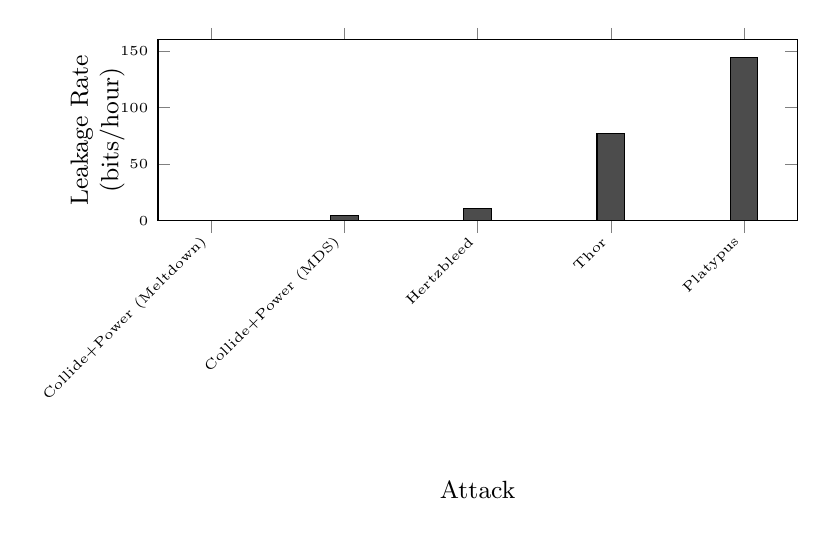
\begin{tikzpicture}
    \begin{axis}[
        ybar,
        symbolic x coords={Collide+Power (Meltdown), Collide+Power (MDS), Hertzbleed, Thor, Platypus},
        xtick=data,
        width=\linewidth*0.8,
        height=\linewidth*0.32,
        xlabel={Attack},
        ylabel={Leakage Rate\\(bits/hour)},
        ymin=0,
        ymax=160,
        x tick label style={
            rotate=45, 
            anchor=east,
            font=\tiny 
        },
        y tick label style={
            font=\tiny 
        },
        bar width=10pt,
        xlabel style={yshift=-0.7cm, font=\small},
        ylabel style={yshift=-0.3cm, align=center, font=\small},
    ]
        \addplot[
        color=black, 
        fill=black!70] coordinates {
            (Collide+Power (Meltdown), 0.136)
            (Collide+Power (MDS), 4.82)
            (Hertzbleed, 10.5)
            (Thor, 76.8)
            (Platypus, 144.7)
        };
    \end{axis}
\end{tikzpicture}
    \caption{\textsc{Thor} leakage rate comparison.}
    \label{fig:thorleakage}
\end{figure}
%
\subsection{Counter-measurement}
\begin{comment}
\textsc{Thor} relies only on precise \textit{timing} measurements. Therefore, it cannot be mitigated by defenses that alter the classification output of NNs, such as adding noise or rounding confidence scores ____. 
Trusted Execution Environment (TEE)-based defenses, such as those performing non-linear computations inside the TEE while offloading linear computations to untrusted sources ____, are also inadequate since we confirmed that the value dependencies of Intel AMX timing that \textsc{Thor} relies on are unaffected by TEE environments like Intel SGX. 
AI workloads demand high speed and efficiency, prompting AI libraries to prioritize performance optimizations. As a result, known constant-time programming techniques are often unsuitable as a defense. For example, masking can help protect weights from leaking but introduces extra computational overhead, increasing both power consumption and execution time.
\end{comment}
\textsc{Thor} relies only on precise \textit{timing} measurements. Thus, it cannot be mitigated by defenses that alter NN classification outputs, such as adding noise or rounding confidence scores ____. Trusted Execution Environment (TEE)-based defenses, like those performing non-linear computations inside the TEE while offloading linear computations to untrusted sources ____, are also inadequate, as the value dependencies of Intel AMX timing that \textsc{Thor} relies on are unaffected by TEE environments like Intel SGX. AI workloads demand high speed and efficiency, prompting AI libraries to prioritize performance optimizations. As a result, known constant-time programming techniques are often unsuitable as a defense. For example, masking can help protect weights from leaking but introduces extra computational overhead, increasing both power consumption and execution time.

A more effective strategy involves introducing response randomness by delaying execution, which disrupts the timing signals relied upon by \textsc{Thor}. However, this approach adds latency to AI applications. Limiting the query rate of the model 
could also slow these attacks, but at the cost of reducing system responsiveness.
Extending detection mechanisms, 
to identify malicious patterns in power and performance characteristics offers a promising defense against \textsc{Thor}.
Lastly, employing homomorphic encryption 
could provide robust protection but comes with substantial computational overhead and performance costs, making it less practical for high-speed AI applications.


%\subsection{Power \& Performance Overhead}
% In an experiment, we measured the time to execute a single AMX multiplication instruction while varying the intervals between consecutive executions. By adjusting the length of these intervals, we identified five distinct execution times, classifying them into performance states. The shortest execution time with the lowest intervals was labeled as the "Warm State," while the longer execution times with higher intervals were classified as "Cold States." 
One mitigation which can be applied through a micro-code update or a software patch is to keep the AMX unit moderately in the Warm State at all times or at least during Intel SGX execution to protect TEEs computation against \textsc{Thor}.
%
This approach is effective because we observed that timing differences dependent on zero values are only significantly measurable when the Intel AMX is in a Cold State. Warm and Cold States introduced here come from an interesting observation in which 
%In an experiment, 
we measured the time to execute a single AMX multiplication instruction while varying the intervals between consecutive executions. By adjusting the length of these intervals, we identified five distinct execution times, classifying them into performance states. The shortest execution time with the lowest intervals was labeled as the Warm State, while the longer execution times with higher intervals were classified as Cold States.  These performance states are shown in Figure~\ref{fig:Performance_Stages}.
However, this mitigation comes with trade-offs in power management and execution speed, as system power limits could be more easily reached, leading to unnecessary throttling of the AMX unit. We measured the power overhead of such defense for \textsc{Thor} and found that depending on the cold vs. warm stage,  the overhead ranges from 2.59\% to 12.33\%. Although this secure design requires more power consumption, it is faster as it keeps the Intel AMX in the highest performance state at all time; this is in contrary to other secure designs for different microarchitectural attacks which almost always incurred a high performance overhead. 
%\textcolor{red}{Todo  quantitatively calculate the AMX latency in warm state over cold state and add numbers here saying how much faster approx.  }

%Although the secure design requires more power consumption, it could be faster in scenarios such as workloads with infrequent multiplications.
\begin{figure}
    \centering
    \begin{tikzpicture}
        \begin{axis}[
            xmin=100, xmax=1000000000,
            ymin=10, ymax=100000,
            xlabel={Interval Delay (Cycle)},
            ylabel={Multiplication Execution\\Time (Cycle)},
            xmode=log, 
            ymode=log,
            log basis x=10, 
            log basis y=10,
            grid=both,
            major grid style={line width=0pt,draw=white!50},
            minor grid style={line width=0pt,draw=white!20},
            font=\scriptsize,
            ylabel style={yshift=0pt, align=center}, 
            width=\linewidth*1,
            height=\linewidth*0.45,
        ]
            \addplot[darkgray, thick] table {Diagrams/Data/warmup.txt};
        \end{axis}
        
        \draw[->, black, thick] (2.1,0.45) -- (1.1,0.45) node[midway, above] {\scriptsize Warm State};
         \node[gray, thick] at (1.05,1.3) {\scriptsize Cold State 1};
         \node[gray, thick] at (2.8,1.7) {\scriptsize Cold State 2};
         \node[gray, thick] at (4.9,1.85) {\scriptsize Cold State 3};
         \node[gray, thick] at (6.4,2.15) {\scriptsize Cold State 4};
         
    \end{tikzpicture}
    \caption{  Performance States of
TMUL and the Secure Recommended Intel AMX Operational State (Warm).}
    \label{fig:Performance_Stages}
\end{figure}

Thus, future research must prioritize the development of effective mechanisms to mitigate the proposed threat vector introduced by AMX and similar technologies while addressing the secure design's performance and power consumption. 

%